% Modified based on Xiaoming Sun's template and https://www.overleaf.com/latex/templates/cs6780-assignment-template/hgjyygbykvrf

\documentclass[a4 paper,12pt]{article}
\usepackage[inner=2.2cm,outer=2.2cm,top=2.5cm,bottom=2.5cm]{geometry}
\usepackage{setspace}
\usepackage[rgb]{xcolor}
\usepackage{verbatim}
\usepackage{subcaption}
\usepackage{fancyhdr}
\usepackage[colorlinks=true, urlcolor=blue, linkcolor=blue, citecolor=blue]{hyperref}
\usepackage{booktabs}
\usepackage{amsmath,amsfonts,amsthm,amssymb}
\usepackage{setspace}
\usepackage{fancyhdr}
\usepackage{lastpage}
\usepackage{extramarks}
\usepackage{indentfirst}
\usepackage{chngpage}
\usepackage{soul,color}
\usepackage{bm}
\usepackage{graphicx,float,wrapfig}
\usepackage{tikz}
\usepackage{makecell}
\setlength{\parindent}{2em}
\usetikzlibrary{positioning}
\usetikzlibrary{arrows,graphs}
\newcommand{\homework}[3]{
   \pagestyle{myheadings}
   \thispagestyle{plain}
   \newpage
   \setcounter{page}{1}
   \noindent
   \begin{center}
   \framebox{
        \vbox{\vspace{2mm}
        \hbox to 6.28in { {\bf Causal and Statistical Inference \hfill} {\hfill {\rm #2} {\rm #3}} }
        \vspace{4mm}
        \hbox to 6.28in { {\Large \hfill #1  \hfill} }
        \vspace{3mm}}
   }
   \end{center}
   \vspace*{4mm}
}
\newcommand\numberthis{\addtocounter{equation}{1}\tag{\theequation}}

% Custom defined operators
\DeclareMathOperator{\Do}{do}
\newcommand{\indep}{\perp \!\!\! \perp}

\begin{document}
\homework{Poster Report: RDD}{Kai Su,}{Qihang Chen}

\textit{All source codes in this poster can be found on \url{https://github.com/sshockwave/RDD_project}.}

\section{Analysis with Baysian Networks}
\subsection{Introduction to RDD}
When the running variable $X$ takes value at different side of a threshold value $t$, there will be a treatment(marked $w=1$) having an effect on the output $Y$ on one side of $X=t$ and no treatment(marked $w=0$) on the other side. Our goal is to measure the average effect $\tau$ solely caused by the treatment. That is, $\tau=E[Y|\Do(W)=1]-E[Y|\Do(W)=0]$.

Such effect appears as a sudden increase or decrease of $y$ in the neighborhood of $X=t$(See Fig.\ref{fig:rddintro}). Therefore, $\tau$ is traditionally estimated using the see effect of $W$. Formally put,

\begin{equation}
   \hat\tau=\lim_{x\to t^+}E[Y|X=x]-\lim_{x\to t^-}E[Y|X=x].\label{eqn:est_lim}
\end{equation}

For simplicity, denote 
\begin{align}
   E[Y|X=t_+]=\lim_{x\to t^+}E[Y|X=x],\\
   E[Y|X=t_-]=\lim_{x\to t^-}E[Y|X=x].
\end{align}

However, we are lack of data near the threshold in most cases, difficult for us to calculate these values on the threshold directly. Thus we need some regression to infer the relation between $X$ and $Y$ so as to predict $E[Y|X=t_+]$ and $E[Y|X=t_-]$.

A common practice is to apply linear regression on both sides. The data near the threshold is more valuable, thus we can set a bandwidth $b$, which is the largest distance where data are taken into account; and a kernel $k$, which assigns weights to data. Denote such an estimator as $\hat\tau(b,k)$.

\begin{figure}[h]
	\centering
   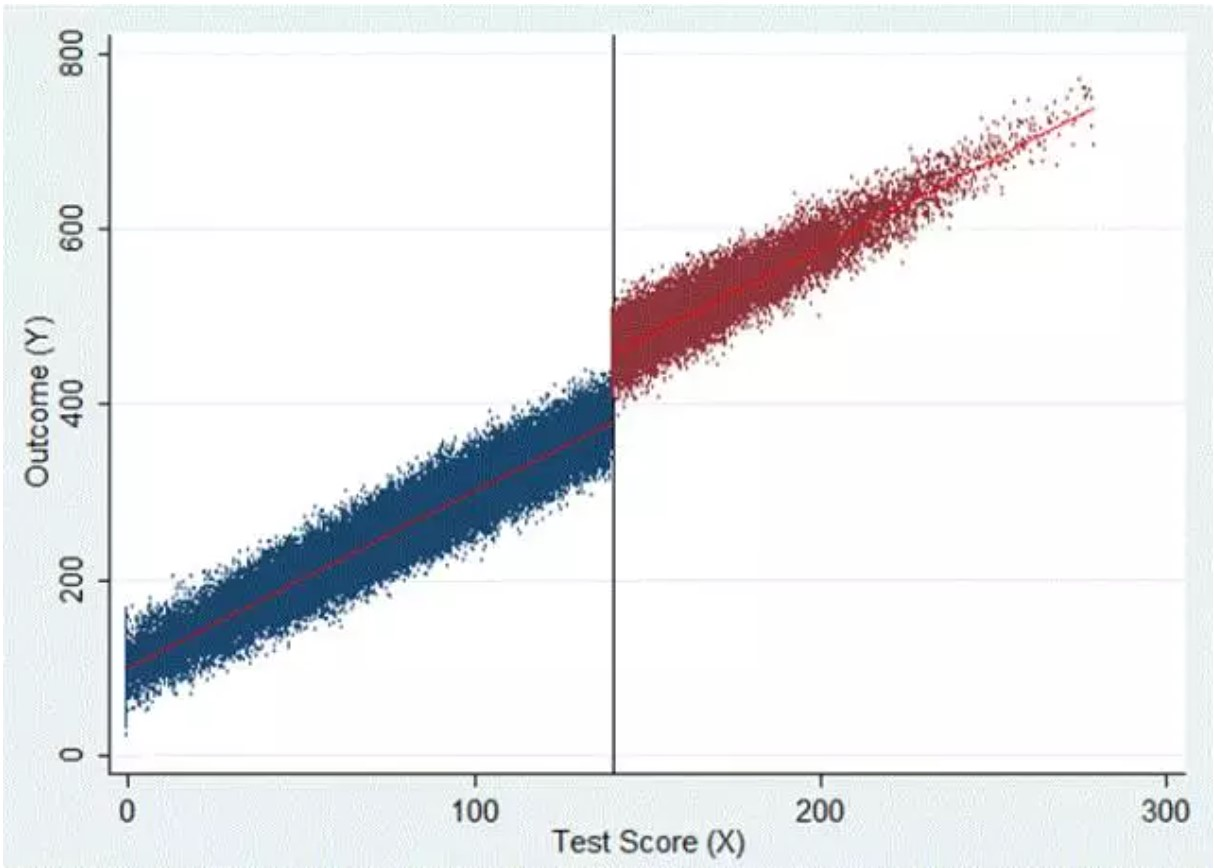
\includegraphics[scale=1]{RDDintro.jpg}
   \caption{An example of dataset in RDD}
   \label{fig:rddintro}
\end{figure}

\subsection{Baysian Networks}
%对应作业第一部分

Basically, running variable $X$ will decide $W$ and affect $Y$; $W$ will have effect on $Y$, as in Fig.\ref{fig:basic_rd_bns}.

\begin{figure}[h]
	\centering
   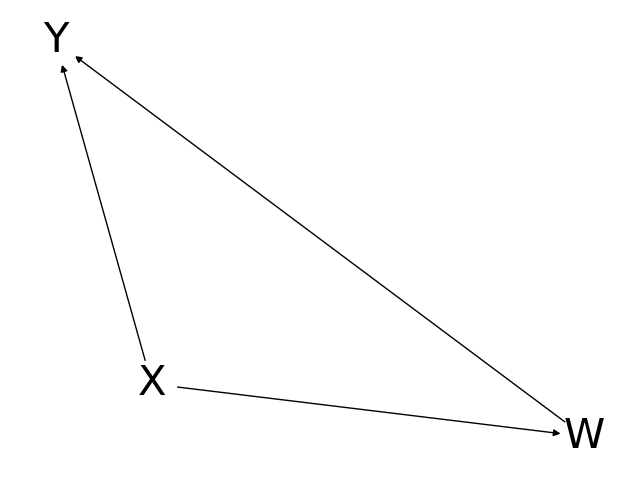
\includegraphics[scale=0.3]{Figure_1.png}
   \caption{The basic BN for RDD}
   \label{fig:basic_rd_bns}
   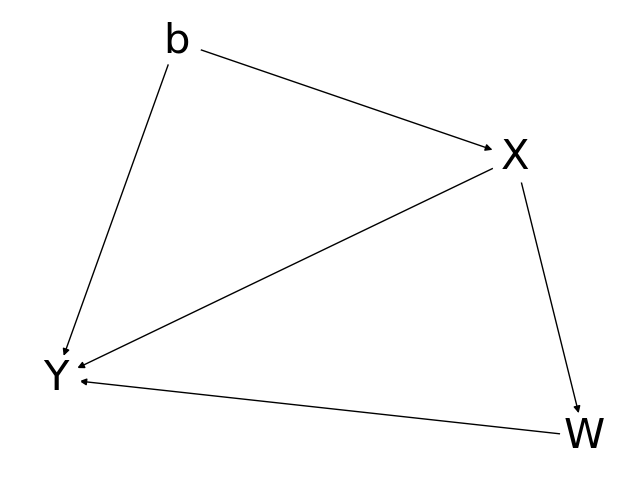
\includegraphics[scale=0.3]{Figure_2.png}
   \caption{BN with bandwidth}
   \label{fig:bn_with_bdw}
\end{figure}

\subsubsection*{Bandwidth}
When the bandwidth is sufficiently small,
\begin{align}
   P(Y|W=0,X=t)\approx P(Y|X=t_-),\\
   P(Y|W=1,X=t)\approx P(Y|X=t_+).
\end{align}

Then
\begin{align}
   \tau&=E[Y|\Do(W=1),X=t]-E[Y|\Do(w=0),X=t]\\
   &\approx E[Y|X=t_+]-E[Y|X=t_-]=\hat\tau,
\end{align}

\noindent proving that the traditional estimation in Eqn.(\ref{eqn:est_lim}) is unbiased.

In contrast, if the bandwidth $b$ is non-negligible, this selection of data specified by $b$ will cause a backdoor path between $X$ and $Y$. (See Fig.\ref{fig:bn_with_bdw}) Then the see effect observed by regression between $X$ and $Y$ is not the true causal effect, leading to a bias.

\subsubsection*{Covariates}
Sometimes there are not only running variables $X$ and $Y$, but also many other variables $Z$, called covariates, may have effect on $Y$. If they are independent with $X$, the regression still works. However in some cases, $Z$ will affect both $X$ and $Y$, creating a backdoor path between $X$ and $Y$. (See Fig.\ref{bn_with_covar})

\begin{figure}[h]
	\centering
	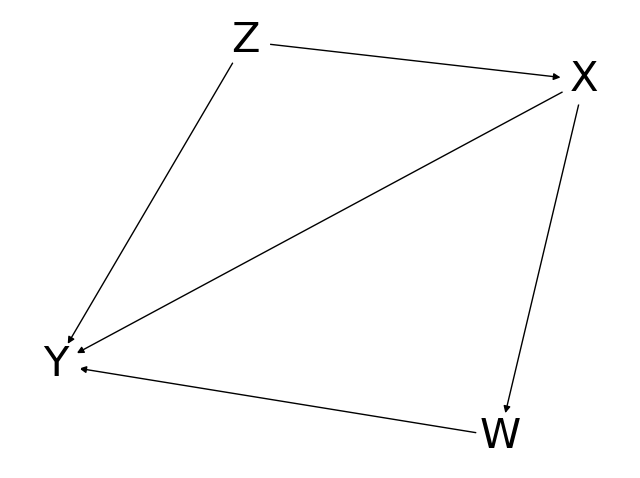
\includegraphics[scale=0.3]{Figure_3.png}
   \caption{BN with covariates}
   \label{bn_with_covar}
	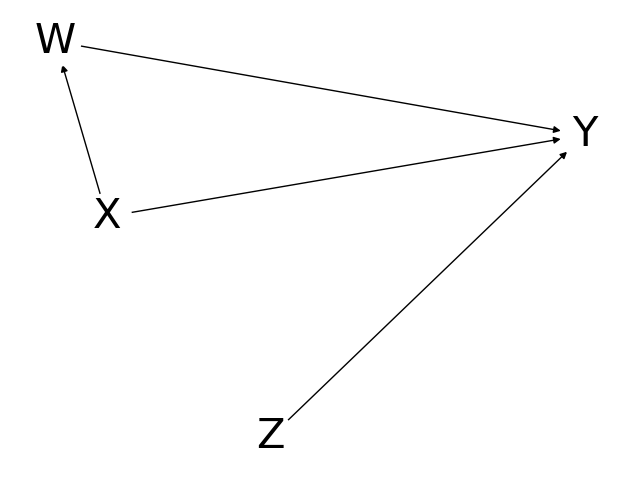
\includegraphics[scale=0.3]{Figure_4.png}
	\caption{Eliminating $Z\rightarrow X$}
	\label{bn_with_covar2}
\end{figure}

\subsection{Obstacles in the BN}
\label{sec:obstacles}
%对应作业第二部分

Under the BN shown in Fig.\ref{fig:bn_with_bdw}, the performance of the estimator $\hat \tau(b,k)$ is restricted by two factors:

\begin{enumerate}
   \item[(a)] Large variance due to lack of data;
   \item[(b)] Bias caused by fitting non-linear $X-Y$ relation with linear regression.
\end{enumerate}

When $b\to 0$, less and less data stay within the bandwidth, so the variance in (a) becomes significant. The bias in (b) converges to $0$ under smoothness assumption on the $X-Y$ relation. The conclusion is opposite when $b\to+\infty$.

If covariates create a backdoor path as shown in Fig.\ref{bn_with_covar2}, the confound effect significantly becomes a source of error in cases with large bandwidth and non-linear $X-Y$ relation.

\section{Experiment and Discussion}

The bandwidth $b$ and the kernel $k$ together decides the weights of data,
yet they are separated into two independent parameters.
The bandwidth focuses on the definition of ``distance'',
and thus allows the reuse of kernels across problems of similar properties but with different scales and units.

Moreover, the final probability distribution of samples supplied to the regression model is a composite outcome of the weights of data and the density of actual data.
Only then can we improve the accuracy of $\hat\tau$ by manipulating $b$ and $k$.
By letting the errors stated in section \ref{sec:obstacles} be the loss function, we get a chain of methods to determine $b$ and $k$:
\begin{enumerate}
   \item Find a bandwidth $b$ which balances between
   \begin{enumerate}
      \item the lack of data;
      \item and bias caused by non-linearity of $X-Y$ relation.
   \end{enumerate}
   \item Find a kernel $k$ which
   \begin{enumerate}
      \item helps to reduce the bias caused by bandwidth;
      \item eliminates the confound effect as much as possible.
   \end{enumerate}
\end{enumerate}

\subsection{Error-minimizing Bandwidth Belection}

In some articles, the method of cross validation is used for selecting an optimal bandwidth.
However, this is not always reliable,
because the samples near the threshold may perform very differently.
Differences in these properties might result in a poor bandwidth for the estimation at the threshold.

If $X-Y$ relation is non-linear,
the curvature of the function $y=y(x)$ varies.
An overestimation of the curvature leads to small bandwidth,
which does not take full advantage of the data.
An underestimation of the curvature leads to large bandwidth,
which might introduce more bias from the non-linear $X-Y$ relation.

Difference of density of data is another issue, particularly in RDD.
Data near the threshold might be under subjective manipulation.
For example, students might work hard not to get below the pass line,
so the number of students who is right below $60$ is much less than the number of students with other scores.
This turbulance in the density of data, again, does not help to select a good bandwidth through cross validation.

Therefore, we propose a method of quantifying the expected error at the cutoff directly, which is an estimation of the two aspects mentioned in section \ref{sec:obstacles}:

\begin{enumerate}
   \item[(a)] Using bandwidth $b$, suppose the linear regression has the result $Y=a(X-t)+b$. We use a formula to calculate the standard derivation of $b$ to represent the expected error caused by lack of data near threshold.
   \item[(b)] First use a quadratic hypothesis function for regression to find out a curve showing approximate quadratic relationship between $X-Y$. This hypothesis function should be unified for all $b$. Then project all the samples onto the curve, use linear regression with bandwidth $b$ and find the difference of value between the two ways of regression on the threshold.
\end{enumerate}

Finally, we find a bandwidth who has least sum of those two kind of errors, which is the optimal bandwidth we need. (See Fig.\ref{table:opt bandwidth})

\begin{figure}[h]
	\centering
	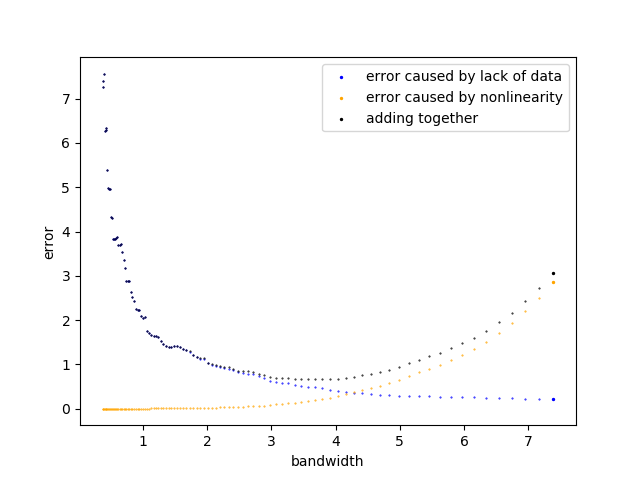
\includegraphics[scale=1]{Figure_5.png}
	\caption{Evaluate error of different bandwidth (on the headstart dataset)}
	\label{table:opt bandwidth}
\end{figure}

\subsection{Using Kernels to Reduce Bias Caused by Bandwidth}

In this section we do not consider covariates.
There are a vast types of kernels.
Triangle and rectangle kernels are used frequently in previous studies.
We extracted some properties from these kernels:
\begin{enumerate}
   \item smooth;
   \item monotonic;
   \item non-zero within the bandwidth, leaving zeros outside.
\end{enumerate}

In common sense, a good kernel is very likely to contain these properties.
So we decided to test against the class of bezier curves,
which is able to mimic most of such functions.

\begin{table}[h]
	\centering
   \begin{tabular}{|c|c|c|c|}
      \hline
      $y=$&$0.2(x-59)^2+2$&$-0.2(x-59)^2-0.4(x-59)+2$&$0.1(x-59)^3+2$\\
      \hline
      Dense middle&case00&case01&case02\\
      \hline
      Sparse middle&case10&case11&case12\\
      \hline
      Dense cutoff&case20&case21&case22\\
      \hline
      Sparse cutoff&case30&case31&case32\\
      \hline
   \end{tabular}
   \caption{$X-Y$ relations and data distributions}
   \label{table:kernels_test}
\end{table}

We designed different $X-Y$ relations and different distributions of samples (See table \ref{table:kernels_test}).
The cutoff is at $X=59$.
Then we randomly generated 500 groups of data and 200 different types of kernels using bezier curves. For each kernel, we calculate the difference of $Y$ at threshold compared with $Y(t)$ by true $X-Y$ relation in those 500 groups of data, and use the average as the benchmark for the kernel.
Then we get the preferred kernel for a fixed bandwidth.

\begin{figure}
   \centering
   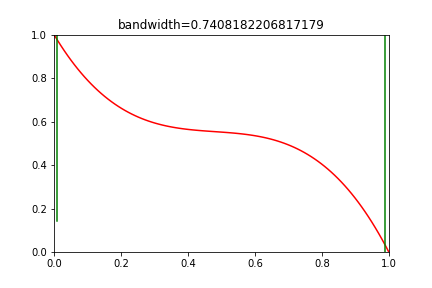
\includegraphics[scale=0.3]{case30_frame0000000.png}
   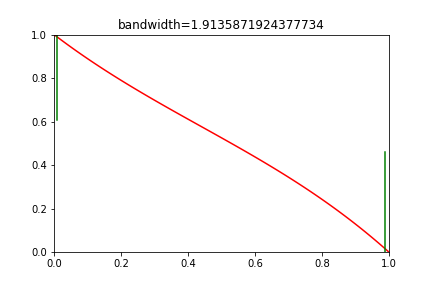
\includegraphics[scale=0.3]{case30_frame0000031.png}
   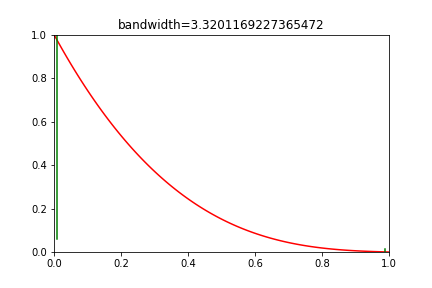
\includegraphics[scale=0.3]{case30_frame0000049.png}
   \caption{Illustrated best kernels under different bandwidths}
   \label{fig:kernels}
\end{figure}
\subsubsection*{Kernels Vary with Bandwidth}

A typical result(case30) is shown in Fig.\ref{fig:kernels}. The $x$-axis is the distance from the cutoff, and the $y$-axis is the weight of the kernel. At a fixed bandwidth, the kernel does not gather around the cutoff at first, but chooses to spread out the weight to larger distance to the cutoff when bandwidth is small.

This initial behavior of the kernel is related to the error mentioned in section \ref{sec:obstacles}(a). The lack of samples cause large uncertainty. Assigning more weight to those farther samples basically equivalents to obtaining more samples, and by doing so, the kernel is able to lower the variance of estimation. As the bandwidth $b$ becomes larger, the weights concentrate to the cutoff to lower the bias caused by the nonlinearity in $X-Y$ relation, corresponding to section \ref{sec:obstacles}(b).

\subsubsection*{Kernels Vary with Density of Data}

Another observation is that, the distribution of samples along $X$ axis really affect the performance of kernels. The reason is the distribution of samples affect the randomness of sampling, thus we need to use the kernel to adjust the sampling method.

Comparing the result in different rows(in html files, can not be shown in pdf), we can find a regular pattern that adding weight on those samples where samples along the $X$ axis are sparse will give better performance. 

It is intuitive to explain this observation. If the samples are evenly distributed, it is easier to infer the information from data. But if some areas on $X$ axis has larger density of samples, giving less weight to them can mimic an evenly distributed set of data. Then the kernel will trend to trust samples in the sparse area.

\subsection{Differences after Adding Covariates}
We generate data by different $X-Y$ relation and different ways that $Z$ affect $X,Y$ (See table \ref{table:kernels_test adding covariates}) where the samples are uniformly distributed.

\begin{table}[h]
   \centering
   \begin{tabular}{ c c c c}
   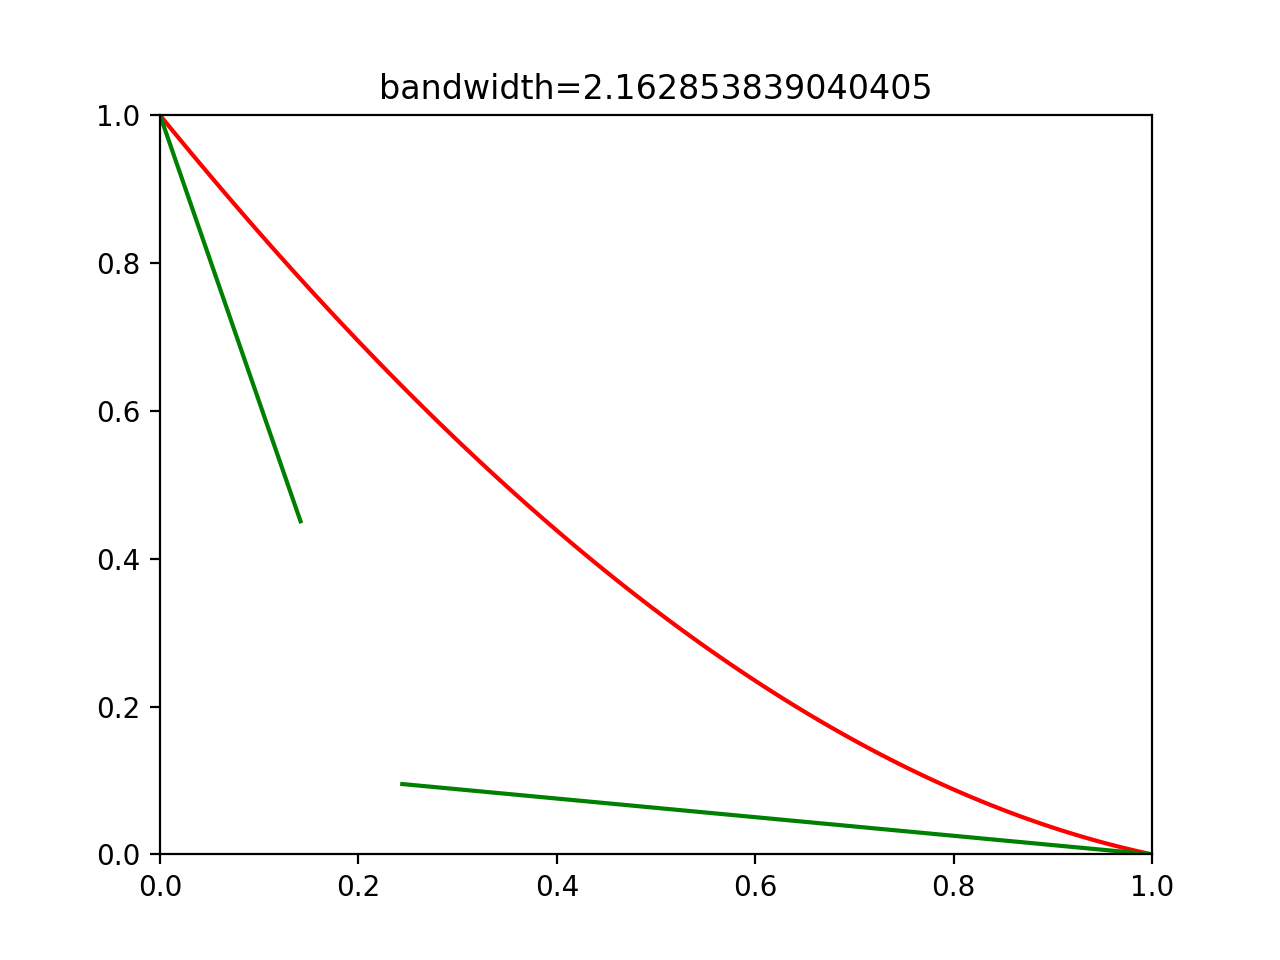
\includegraphics[scale=0.2]{case41_frame0000035.png}
   &
   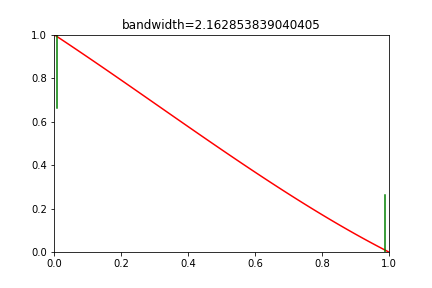
\includegraphics[scale=0.24]{casez01_frame0000035.png}
   &
   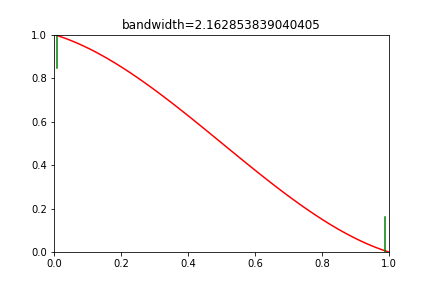
\includegraphics[scale=0.24]{casez11_frame0000035.png}
   &
   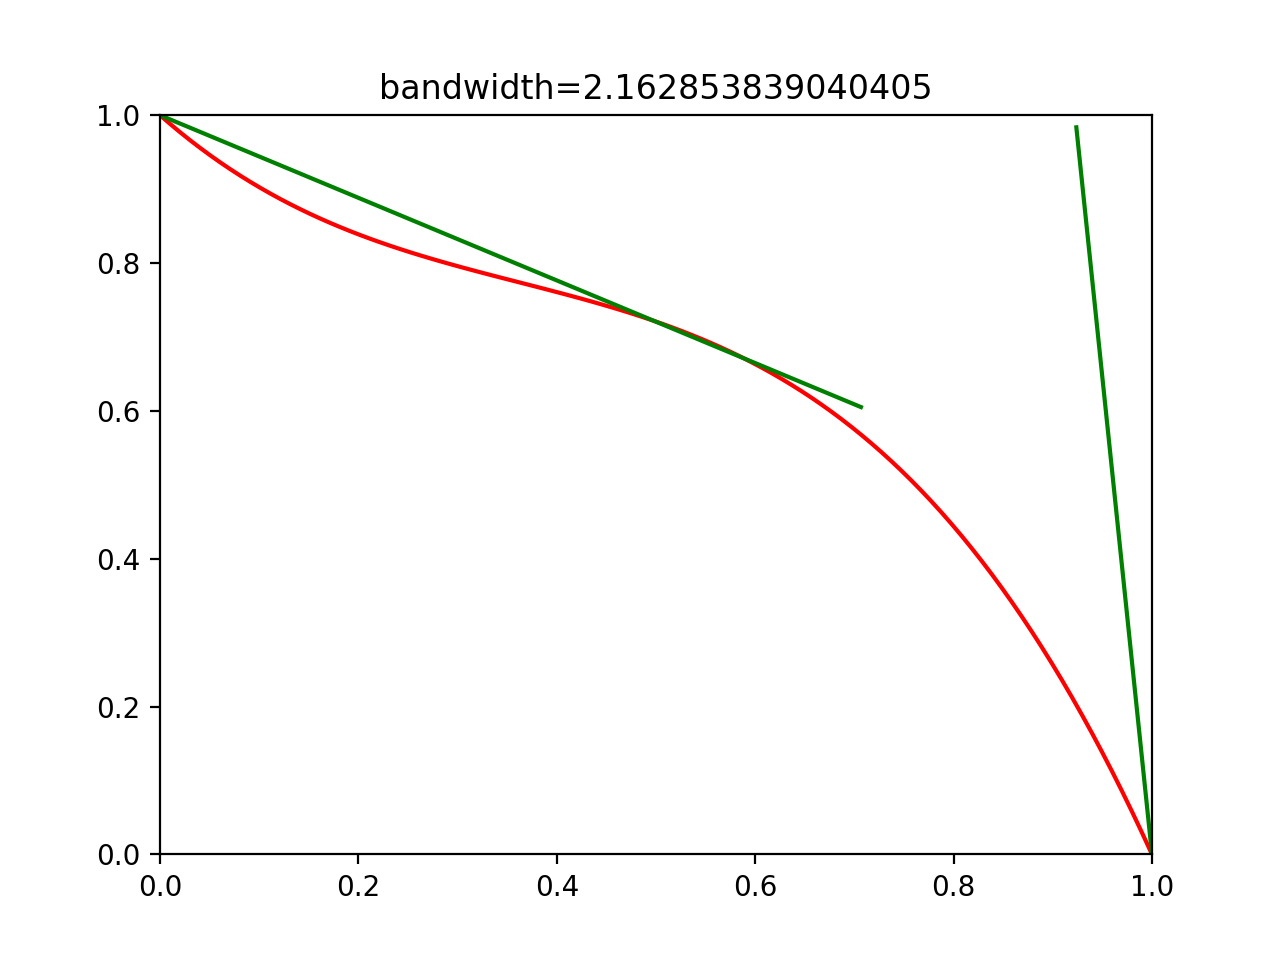
\includegraphics[scale=0.2]{casez21_frame0000035.png}
   \\
   case41&casez01&casez11&casez21\\
   \end{tabular}
	\caption{Illustrated best kernels under different ways of adding covariates with $b=2.1628$}
	\label{fig:kernels2}
\end{table}

After adding covariates, there will be another backdoor path caused by $Z$, and the perfomance of kernels becomes different (See Table \ref{fig:kernels2}). This tells us that covariates do have impact on the result of estimation and our selection of kernels should concern the effect of covariates.

\begin{table}[h]
	\centering
	\begin{tabular}{|c|c|c|c|}
		\hline
		$f(x)=$&$0.2(x-59)^2+2$&$-0.2(x-59)^2-0.4(x-59)+2$&$0.1(x-59)^3+2$\\
		\hline
		\makecell{$x=x_0$\\$y=f(x)$}&case40&case41&case42\\
		\hline
		\makecell{$x=x_0+z$\\$y=f(x)+0.3z$}&casez00&casez01&casez02\\
		\hline
		\makecell{$x=x_0+z^2$\\$y=f(x)+0.3z$}&casez10&casez11&casez12\\
		\hline
		\makecell{$x=x_0+z$\\$y=f(x)+0.5z^2$}&casez20&casez21&casez22\\
		\hline
	\end{tabular}
	\caption{$X-Y$ relations and ways of adding $Z$}
	\label{table:kernels_test adding covariates}
\end{table}

\subsection{Beyond the Kernel: Eliminating the Confound Effect}

This section discusses the feasibility of eliminating the confound effect caused by covariates using bandwidths and kernels.

Let $P(*)$ be the density of data,
and $P'(*)$ be the probability distribution supplied to the regression model.

Let $\omega(x)$ be the random variable representing the nomalized weight of samples located at $x$.
By the definition of bandwidths and kernels,
the weight before normalization for $x$ is

\begin{equation}
   \omega'(x)=\begin{cases}
      k\left(\frac{\left|x-t\right|}{b}\right)&\left|x-t\right|\le b\\
      0&\left|x-t\right|>b
   \end{cases}.
\end{equation}

After normalization,

\begin{equation}
   \omega(x)=\frac{\omega'(x)}{\sum_{x'}\omega'(x')P(x')}.
\end{equation}

Then $P'$ is well-defined by $P'(x,*)=\omega(x)P(x,*)$, since

\begin{align}
   \sum P'(*)=&\sum_xP'(x)\\
   =&\sum_x\omega(x)P(x)\\
   =&\sum_x\frac{\omega'(x)P(x)}{\sum_{x'}\omega'(x')P(x')}\\
   =&1.
\end{align}

Removing $Z\to X$ from Fig.\ref{bn_with_covar} is adding an independence relation between $X$ and $Z$,
which requires

\begin{align}
   P'(x,z)=&P'(x)P'(z)\\
   \omega(x)P(x,z)=&\omega(x)P(x)P'(z)\\
   P(x,z)=&P(x)P'(z)\label{eqn:indep}\\
   \sum_x P(x,z)=&\sum_xP(x)P'(z)\\
   P(z)=&P'(z)\label{eqn:z_zpai}
\end{align}

Combining Eqn.(\ref{eqn:indep})(\ref{eqn:z_zpai}), $P(x,z)=P(x)P(z)$.
Therefore, $Z\to X$ can be removed only if $X\indep Z$ at the very beginning.

If we try to remove $Z\to Y$ instead, then $Y\indep Z\mid X$.

\begin{align}
   P'(y,z\mid x)=&P'(y\mid x)P'(z\mid x)\\
   P'(x,y,z)P'(x)=&P'(x,y)P'(x,z)\\
   (\omega(x)P(x,y,z))(\omega(x)P(x))=&(\omega(x)P(x,y))(\omega(x)P(x,z))\\
   P(x,y,z)P(x)=&P(x,y)P(x,z)\\
   P(y,z\mid x)=&P(y\mid x)P(z\mid x),
\end{align}

giving that $Y\indep Z\mid X$ initially.

In conclusion, the confound effect cannot be eliminated by simply using bandwidths and kernels.
To correctly identify $P(y\mid\hat x)$,
one must assign the weights according to $Z$, too.

\begin{align}
   P'(y\mid x)=&P(y\mid \hat x)\\
   \frac{P'(x,y)}{P'(x)}=&\sum_z P(y\mid \hat x,z)P(z\mid \hat x)\\
   \frac{\sum_z \omega(x,z)P(x,y,z)}{\sum_z \omega(x,z)P(x,z)}=&\sum_z P(y\mid x,z)P(z)
\end{align}

Thus we only need to find a set of weights that satisfies such equation.
A deeper look requires more discussion and will be omitted.

In particular,
if $Y$ is linear with respect to $X$ and $Z$,
the parameters in $Y=X\alpha+Z\beta+\varepsilon$ can be obtained by linear regression,
thus the do effect can be easily estimated.
However, this is not necessary, since the confound effect never shows up in the estimation of treatment in this case.

\end{document}
